\documentclass{article}
\iffalse
This file is protected by Copyright. Please refer to the COPYRIGHT file
distributed with this source distribution.

This file is part of OpenCPI <http://www.opencpi.org>

OpenCPI is free software: you can redistribute it and/or modify it under the
terms of the GNU Lesser General Public License as published by the Free Software
Foundation, either version 3 of the License, or (at your option) any later
version.

OpenCPI is distributed in the hope that it will be useful, but WITHOUT ANY
WARRANTY; without even the implied warranty of MERCHANTABILITY or FITNESS FOR A
PARTICULAR PURPOSE. See the GNU Lesser General Public License for more details.

You should have received a copy of the GNU Lesser General Public License along
with this program. If not, see <http://www.gnu.org/licenses/>.
\fi

% TODO: Version numbers?
\usepackage{graphicx}
\graphicspath{ {figures/} }
\usepackage{fancyhdr}
\usepackage{colortbl}
\usepackage[margin=.75in]{geometry}
\pagestyle{fancy}
\lhead{Matchstiq BSP Case Study}
\rhead{ANGRYVIPER Team}
\definecolor{drkgreen}{rgb}{0,.6,0}
\renewcommand{\headrulewidth}{0pt}
\definecolor{blue}{rgb}{.7,.8,.9}
\begin{document}
\section*{Matchstiq BSP Case Study}
  When each new platform is brought into the OpenCPI framework, there is some work that needs to be done.  The Matchstiq-Z1 platform has many of similarities to the Zedboard platform but there was still a large amount of work that needed to be done to implement this platform.

  \subsection*{Matchstiq-Z1 Platform Block Diagrams}
    \begin{figure}[ht]
      \centerline{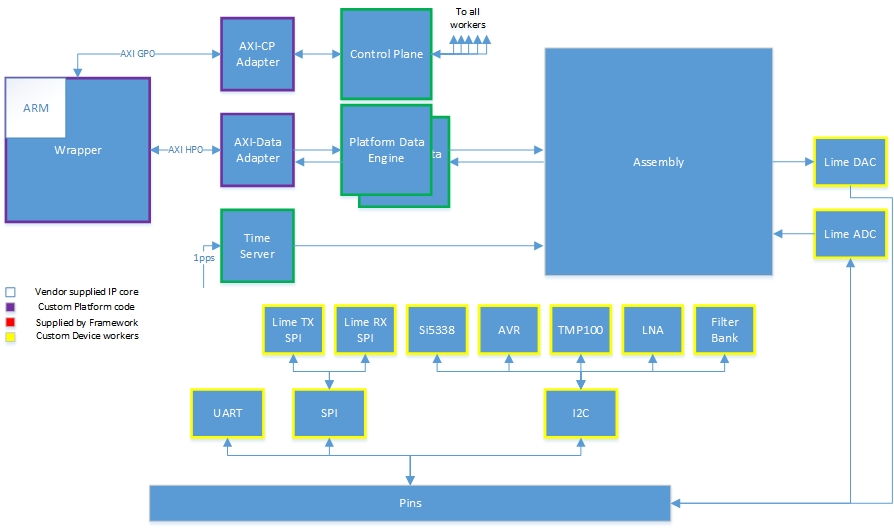
\includegraphics[scale=0.7]{matchstiq_BSP_toplevel}}
      \caption{Top Level Block Diagram}
      \label{fig:top}
    \end{figure}
    \vspace{65 mm}
    \begin{figure}[ht]
      \centerline{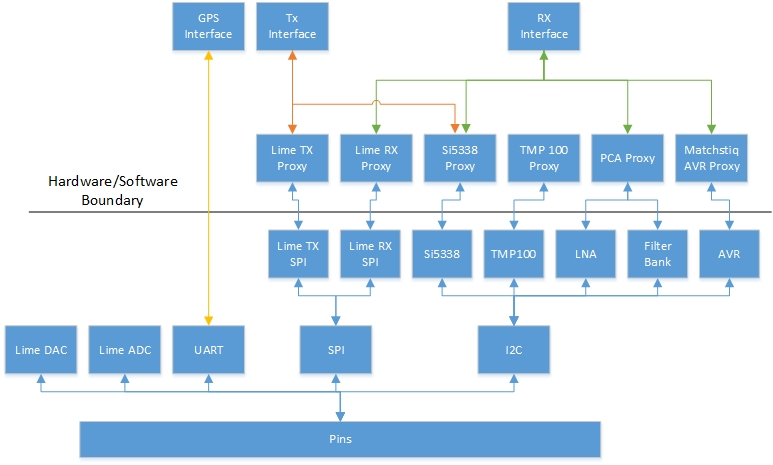
\includegraphics[scale=0.7]{matchstiq_BSP_worker}}
      \caption{Workers Block Diagram}
      \label{fig:top}
    \end{figure}
    \vspace{25 mm}

\section*{Petalinux}

  The first task that needs to be completed is to install the OpenCPI version of Petalinux onto the platform.  In order to boot the platform on the Matchstiq-Z1, there are three things that are needed on the SD card: Device tree, Linux kernel, and the root filesystem.  The First Stage Boot Loader for the Matchstiq is located in flash and was left alone for our implementation.\\

  \noindent There are environment variables that U-Boot (second stage boot loader) use to load files from the SD card into memory to boot the processor.  The original Matchstiq-Z1 SD card image had created a kernel with a small root file system embedded within the kernel. This used different U-boot settings and we had to edit these settings to boot our version. On the Matchstiq-Z1, these U-Boot variables are located on the second partition of the SD card. This is important to keep in mind when trying to create new SD cards for the Matchstiq-Z1.  \\

  \noindent There needs to be a Ethernet connection on the platform.  This is used for development purposes for an NFS mount of the framework and workers to be deployed on the target system.  The Matchstiq-Z1 does not have a Ethernet port, so we use a USB to Ethernet adapter.  We needed to build in support for this device into the Petalinux kernel.  There also needed to be an edit to the Zedboard device tree to support USB on-the-go.  This change was also added to the Zedboard build as well.

\section*{Cross Compiler}

  When the Matchstiq-Z1 was being brought into the framework, the Zedboard platform work had already integrated the cross compiler for Zynq into OpenCPI.  Had this not been the case there would need to be work done to integrate a cross compiler into the framework.

\section*{Device Workers}
  The platform has a set of devices that are connected to the FPGA.  The below device workers needed to be created to give users access to the functionality of these devices.

  \subsection*{I2C Bus}
    There are several devices connected to the I2C bus, the peripherals and their slave addresses were known from the Epiq documentation.  The order and the values of the register settings were reverse engineered by monitoring the I2C bus with a bus analyzer while using Epiq's provided API.  \\

    The I2C connected devices are: SI5338 clock generator, TMP100 temperature sensor, AVR microcontroller, a low noise amplifier, and a RF filter bank.  A device worker and a  proxy worker was developed for each of these peripherals.

  \subsection*{SPI Bus}
    There is a single slave SPI connection on the Matchstiq-Z1 platform connecting to the LMS6002D transceiver for control to the configuration registers of the transceiver.  A device worker and a device proxy needed to be implemented for this device, this was reused from the Zedboard platform.

  \subsection*{GPS UART}
    There is a GPS receiver on the Matchstiq-Z1 that communicates with the FPGA over UART.  A device worker and a device proxy needed to be implemented for this device.

  \subsection*{DAC/ADC}
    There are 12 bit RX and TX data lines to move the I/Q samples from the LMS6002D to the FPGA.  A device worker needed to be written for each of these interfaces.

\section*{HDL Platform}
  The device workers that are described above are instantiated in the container.  The ARM processing system needed to be instantiated into the platform and configured in the correct way. This was a non trivial task to learn how to do but was reused from the Zedboard platform.

  \subsection*{Control Plane Integration}
    The control plane modules are connected to General Purpose AXI port 0 on the ARM processor.  An adapter needed to be written to take data being streamed to the FPGA via AXI to be passed to the HDL framework.  Driver software also needed to be written for the processor to move data from the ARM processor down to the FPGA.  This driver was reused from the Zedboard platform.


  \subsection*{Data Plane Integration}
    The data plane modules are connected to a High performance AXI port on the ARM processor.  An adapter needed to be written to take data being streamed to the FPGA via AXI to be passed to the HDL framework.  Driver software also needed to be written for the processor to move data from the ARM processor down to the FPGA.  This driver was reused from the Zedboard platform.

\section*{Common interfaces}
  Each radio platform will have a common generic software interface for receive and transmit.  These interfaces are documented in the workers data sheets.  The workers for each of these interfaces needed to be implemented on the Matchstiq-Z1 platform.

\end{document}
